\documentclass[sigconf,nonacm]{acmart}

\usepackage[utf8]{inputenc}
\usepackage[T1]{fontenc}  % Melhor suporte para acentuação em português
\usepackage{graphicx}
\usepackage{balance}
\usepackage{booktabs} % Melhor formatação de tabelas
\usepackage{amsmath}  % Suporte para fórmulas matemáticas avançadas
\usepackage{microtype} % Melhoria tipográfica

\begin{document}

\title{Métodos clássicos de exploração de filtros de textura para classificação de imagens médicas}


\author{Luan de Oliveira Magalhães}
\email{luansesi3@gmail.com}
\affiliation{%
  \institution{Departamento de Informática\\Universidade Federal do Paraná}
  \city{Curitiba}
  \state{Paraná}
  \country{Brasil}
}

\author{Raul José Silvério da Silva}
\email{raul.silverio@ufpr.br}
\orcid{0009-0006-5091-1584}
\affiliation{%
  \institution{Departamento de Informática\\Universidade Federal do Paraná}
  \city{Curitiba}
  \state{Paraná}
  \country{Brasil}
}

\author{Vinícius Lázaro Bartolomeu}
\email{vinicius.bartolomeu@ufpr.br}
\affiliation{%
  \institution{Departamento de Informática\\Universidade Federal do Paraná}
  \city{Curitiba}
  \state{Paraná}
  \country{Brasil}
}

\begin{abstract}
  Esse trabalho investiga o impacto de diferentes configurações de filtros de textura para a classificação de imagens médicas, com foco no uso de métodos clássicos de visão computacional.
  A pesquisa analisa o dataset público \textit{medmnist}, com foco na base de dados \textit{PneumoniaMNIST} que contém imagens de raio-X de tórax, e avalia o desempenho de diferentes filtros de textura na extração de características relevantes para a classificação de imagens.
  O estudo utiliza uma abordagem de aprendizado de máquina, aplicando técnicas de pré-processamento e extração de características, seguido por algoritmos de classificação.
\end{abstract}

\keywords{Visão Computacional, Extração de Características, Classificação, Machine Learning}

\maketitle

\section{Introdução}
A classificação de imagens médicas é uma tarefa desafiadora e crucial na área da saúde, com o objetivo de auxiliar profissionais médicos na detecção e diagnóstico de doenças. A análise de imagens médicas, como raios-X, tomografias e ressonâncias magnéticas, requer técnicas avançadas de processamento de imagem e aprendizado de máquina para extrair informações relevantes e realizar classificações precisas.

Neste contexto, os filtros de textura desempenham um papel fundamental na extração de características, permitindo a identificação de padrões e texturas presentes nas imagens. Esses filtros são projetados para capturar informações sobre a estrutura e a distribuição de intensidades de pixel, fornecendo uma representação mais rica das imagens.

Neste trabalho, investigamos o impacto de diferentes configurações de filtros de textura na classificação de imagens médicas, com foco no uso de métodos clássicos de visão computacional. Utilizamos o dataset público \textit{medmnist}, que contém uma variedade de imagens médicas, e avaliamos o desempenho de diferentes filtros de textura na extração de características relevantes para a classificação.


\section{Fundamentação Teórica}

\subsection{Métricas de Avaliação}
Para avaliar o desempenho dos filtros, foram utilizadas as seguintes métricas:

\begin{itemize}
  \item \textbf{Acurácia}: Proporção de previsões corretas em relação ao total de previsões. 
  \[
  \text{Acurácia} = \frac{\text{VP} + \text{VN}}{\text{VP} + \text{VN} + \text{FP} + \text{FN}}
  \]
\end{itemize}

Onde VP = Verdadeiros Positivos, VN = Verdadeiros Negativos, FP = Falsos Positivos e FN = Falsos Negativos.

\subsection{Filtros de Gabor}

Os filtros de Gabor são amplamente utilizados para análise de textura em imagens médicas devido à sua capacidade de capturar informações de frequência e orientação em diferentes escalas \cite{texture_feature_humeau_2019}. Estes filtros são particularmente eficazes na identificação de bordas e padrões repetitivos em imagens, sendo inspirados no funcionamento do sistema visual humano.

A principal vantagem dos filtros de Gabor é sua capacidade de decompor uma imagem em componentes que representam diferentes orientações e escalas, permitindo uma análise detalhada das texturas presentes. Esta característica os torna particularmente úteis para a análise de imagens médicas, onde pequenas variações de textura podem indicar a presença de patologias.

O filtro de Gabor é definido por uma função gaussiana modulada por uma onda senoidal, permitindo a extração de características de frequência e orientação \cite{texture_feature_humeau_2019}. Um filtro de Gabor 2D pode ser calculado como:

\[
G_{\sigma,f_0,\phi}(x,y) = \exp\left(-\frac{1}{2} \left(\frac{x'^2}{\sigma_x^2} + \frac{y'^2}{\sigma_y^2}\right)\right) \cos\left(2\pi f_0 x' + \phi\right),
\]

onde \(\sigma_x\) e \(\sigma_y\) são as escalas do envelope Gaussiano (desvios padrão) nas direções \(x\) e \(y\), respectivamente. \(f_0\) e \(\phi\) são, respectivamente, a frequência e a fase da onda senoidal. \(x'\) e \(y'\) são dados por:

\[
\begin{aligned}
x' &= x \cos(\theta) + y \sin(\theta), \\
y' &= -x \sin(\theta) + y \cos(\theta).
\end{aligned}
\]
onde \(\theta\) é a orientação do filtro.

\subsection{Filtro Laplaciano de Gaussiana (LoG)}

O filtro de Laplaciano de Gaussiana (LoG) é uma técnica clássica de detecção de bordas que combina a suavização de uma imagem com um operador Laplaciano, permitindo a identificação de regiões com alta variação de intensidade.

A formulação matemática do filtro LoG em duas dimensões é dada por:

\[
\text{LoG}(x, y) = -\frac{1}{\pi\sigma^4}\left(1 - \frac{x^2 + y^2}{2\sigma^2}\right)e^{-\frac{x^2 + y^2}{2\sigma^2}}
\]

onde \(\sigma\) representa o desvio padrão do filtro gaussiano.

Porém, um filtro Gaussiano 2D pode ser
substituído por dois filtros Gaussianos 1D,
que são mais rápidos:
\[
G(x,y) = \frac{1}{2\pi\sigma^2}e^{-\frac{x^2 + y^2}{2\sigma^2}} 
\]
\[
G(x,y) = G(x)G(y)
\]
onde \(G(x)\) e \(G(y)\) são os filtros gaussianos unidimensionais aplicados nas direções \(x\) e \(y\), respectivamente.



\subsection{Segmentação por Agrupamento}

A segmentação por agrupamento, como o algoritmo K-means, é uma técnica não supervisionada que permite dividir uma imagem em regiões com características similares. No contexto deste trabalho, utilizamos o K-means para agrupar regiões da imagem com base nas características extraídas pelos filtros de textura, permitindo a identificação de áreas com padrões texturais semelhantes.

\section{Descrição dos Conjuntos de Dados}
\subsection{MedMNIST - PneumoniaMNIST}

O dataset \textit{PneumoniaMNIST} \cite{medmnistv1_2021} é uma coleção de imagens de raios-X de tórax, contendo 5.856 imagens, sendo 4.708 de treinamento, 524 de validação, e 624 imagens de teste. As imagens são rotuladas como "normal" ou "pneumonia", representando a presença ou ausência da doença.

Este conjunto de dados é particularmente relevante para nossa pesquisa, pois a pneumonia frequentemente se manifesta como opacidades e consolidações nos raios-X de tórax, criando padrões texturais distintos que podem ser capturados por filtros adequados. As imagens utilizadas possuem dimensionalidade de 64x64 pixels para facilitar o processamento, mantendo informações suficientes para a análise de textura.

\subsection{Amostragem Experimental e Pré-processamento}
Para um experimento controlado, extraímos do conjunto original uma amostragem balanceada:

\begin{table}[h]
  \centering
  \caption{Amostragem utilizada nos experimentos}
  \label{tab:experimental_splits}
  \resizebox{0.45\textwidth}{!}{%
    \begin{tabular}{ccc}
      \toprule
      \textbf{Conjunto}     & \textbf{Imagens Selecionadas} & \textbf{Proporção por Classe}            \\
      \midrule
      Treinamento          & 200                           & \(\approx\) 50\% normal / 50\% pneumonia \\
      Teste                & 200                           & \(\approx\) 50\% normal / 50\% pneumonia \\
      \bottomrule
    \end{tabular}
  }
\end{table}

\section{Metodologia}

\subsection{Pré-processamento das Imagens}

As imagens foram normalizadas utilizando a função StandardScaler do scikit-learn, que aplica a normalização Z-score. Essa técnica é fundamental para garantir que todas as características tenham a mesma escala, evitando que características com magnitudes maiores dominem o processo de classificação.
A normalização Z-score é calculada como:
\[
z = \frac{x - \mu}{\sigma}
\]
onde \(x\) é o valor original, \(\mu\) é a média e \(\sigma\) é o desvio padrão. Essa normalização é aplicada a cada pixel da imagem, garantindo que os dados estejam centrados em torno de zero e tenham uma variância unitária.

\subsection{Estratégia de Ajuste de Filtros}

A estratégia de ajuste de filtros foi realizada utilizando uma abordagem sistemática, onde diferentes configurações de filtros de textura foram aplicadas às imagens do dataset. 

\subsection{Banco de Filtros Proposto}

Nossa abordagem utiliza um banco de filtros composto por:

\begin{itemize}
  \item \textbf{Filtros de Gabor:} Implementamos 12 filtros de Gabor com diferentes configurações, combinando:
  \begin{itemize}
    \item Quatro orientações: 0°, 45°, 90° e 135°
    \item Três escalas (lambda): 3, 6 e 12
  \end{itemize}
  \item \textbf{Filtros Laplacianos de Gaussiana (LoG):} Implementamos três filtros LoG com diferentes escalas (sigma = 1, 2 e 4) para capturar características circulares e bordas em diferentes escalas.
\end{itemize}

Esta combinação de filtros permite capturar uma ampla gama de características texturais nas imagens médicas, desde bordas finas e detalhes até estruturas maiores e padrões mais amplos.

\subsection{Extração de Características}

Para a extração de características, dividimos cada imagem em janelas não sobrepostas de tamanho 5×5 pixels. Para cada janela, calculamos a média da resposta de cada filtro, gerando um vetor de características de dimensão igual ao número de filtros (15 no total).

Esta abordagem baseada em janelas permite uma análise local das texturas, preservando informações espaciais importantes para a classificação, ao mesmo tempo em que reduz a dimensionalidade dos dados e aumenta a robustez a ruídos.

\subsection{Segmentação por Textura}

Utilizamos o algoritmo K-means para agrupar regiões da imagem com base nas características extraídas. Definimos o número de clusters como 4, representando diferentes padrões texturais presentes nas imagens. Para garantir a robustez do agrupamento, as características foram padronizadas antes da aplicação do K-means, usando a técnica de padronização Z-score:

\[
z = \frac{x - \mu}{\sigma}
\]

onde \(x\) é o valor original, \(\mu\) é a média e \(\sigma\) é o desvio padrão.

\subsection{Análise Multi-escala}

Implementamos duas abordagens para análise multi-escala:

\begin{itemize}
  \item \textbf{Filtros em múltiplas escalas:} Aplicação direta de filtros com diferentes parâmetros de escala na imagem original.
  \item \textbf{Pirâmide de imagens:} Aplicação de filtros em versões reduzidas da imagem, capturando características em diferentes níveis de detalhe.
\end{itemize}

A abordagem de pirâmide de imagens consiste em aplicar filtros de Gabor e LoG à imagem original e, em seguida, reduzir a resolução da imagem (downsampling) após aplicação de um filtro gaussiano para evitar aliasing. Este processo é repetido para três níveis de resolução, permitindo a captura de características em diferentes escalas.

\section{Resultados e Análises}

Nesta seção, apresentamos os resultados obtidos com a aplicação dos filtros de textura e discutimos suas implicações para a classificação de imagens médicas.

\subsection{Análise Qualitativa dos Filtros}

A aplicação dos filtros de Gabor e LoG nas imagens de raio-X revelou padrões texturais distintos entre casos normais e casos de pneumonia. Os filtros de Gabor com orientações horizontais (0°) e verticais (90°) mostraram-se particularmente eficazes na detecção de opacidades pulmonares características da pneumonia.

A Figura \ref{fig:filtros_pneumonia} ilustra a aplicação dos filtros em uma imagem de raio-X com pneumonia, mostrando as respostas dos filtros de Gabor em diferentes orientações e escalas, bem como do filtro LoG. Podemos observar que os filtros ressaltam diferentes características texturais da imagem, permitindo uma análise mais detalhada das estruturas presentes.
\begin{figure}[h]
  \centering
  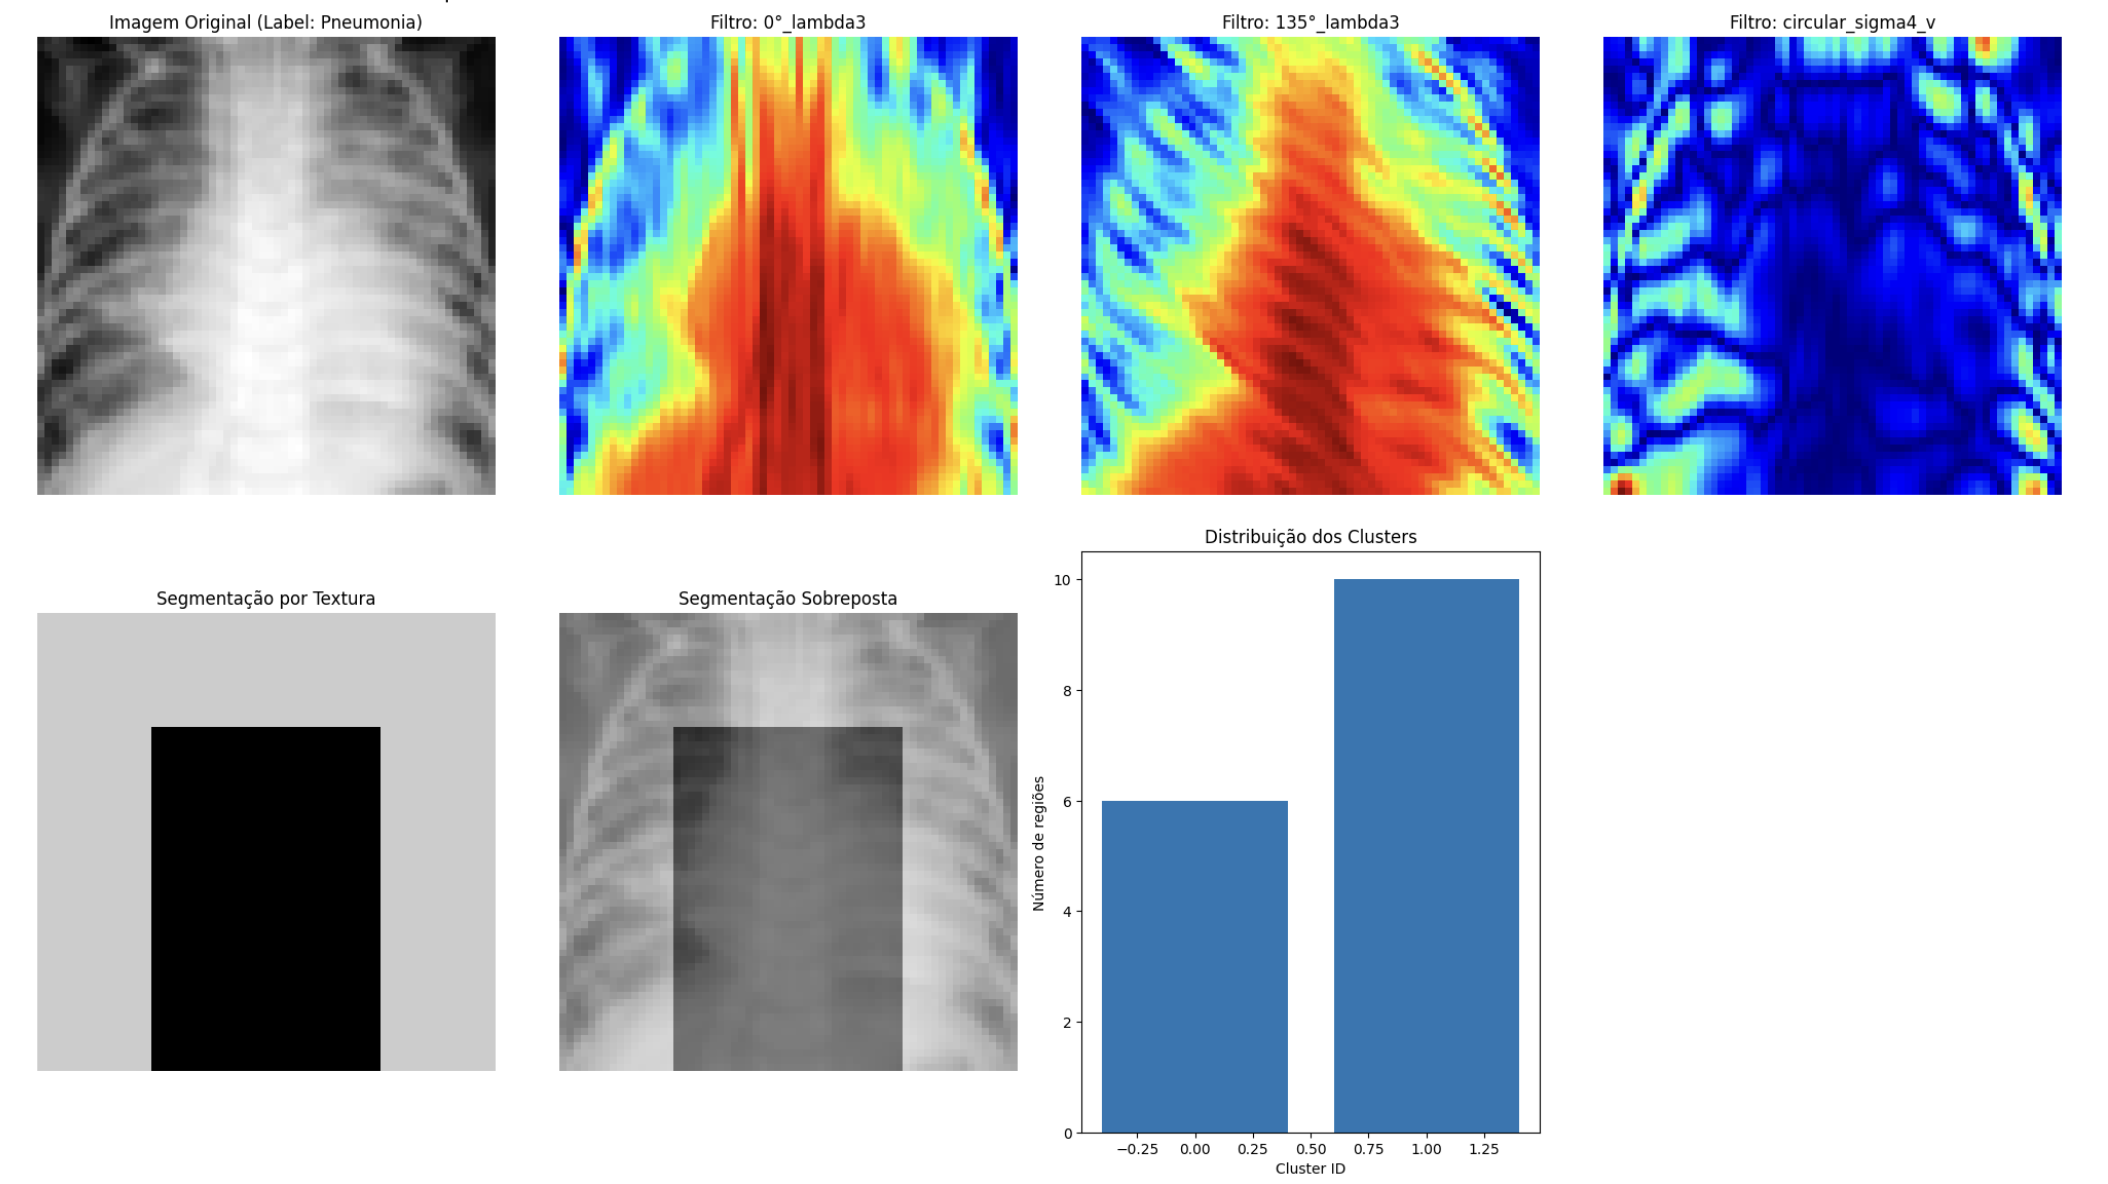
\includegraphics[width=1\linewidth]{../images/filtros_pneumonia.png}
  \caption{Respostas dos filtros de Gabor e LoG aplicados a uma imagem de raio-X com pneumonia.}
  \label{fig:filtros_pneumonia}
\end{figure}

Em contraste, as imagens normais apresentaram respostas mais homogêneas aos filtros, com menor variação de intensidade e padrões texturais menos complexos. A Figura \ref{fig:filtros_normal} ilustra a aplicação dos filtros em uma imagem normal, evidenciando a diferença nas respostas dos filtros em comparação com os casos de pneumonia.

\begin{figure}[h]
  \centering
  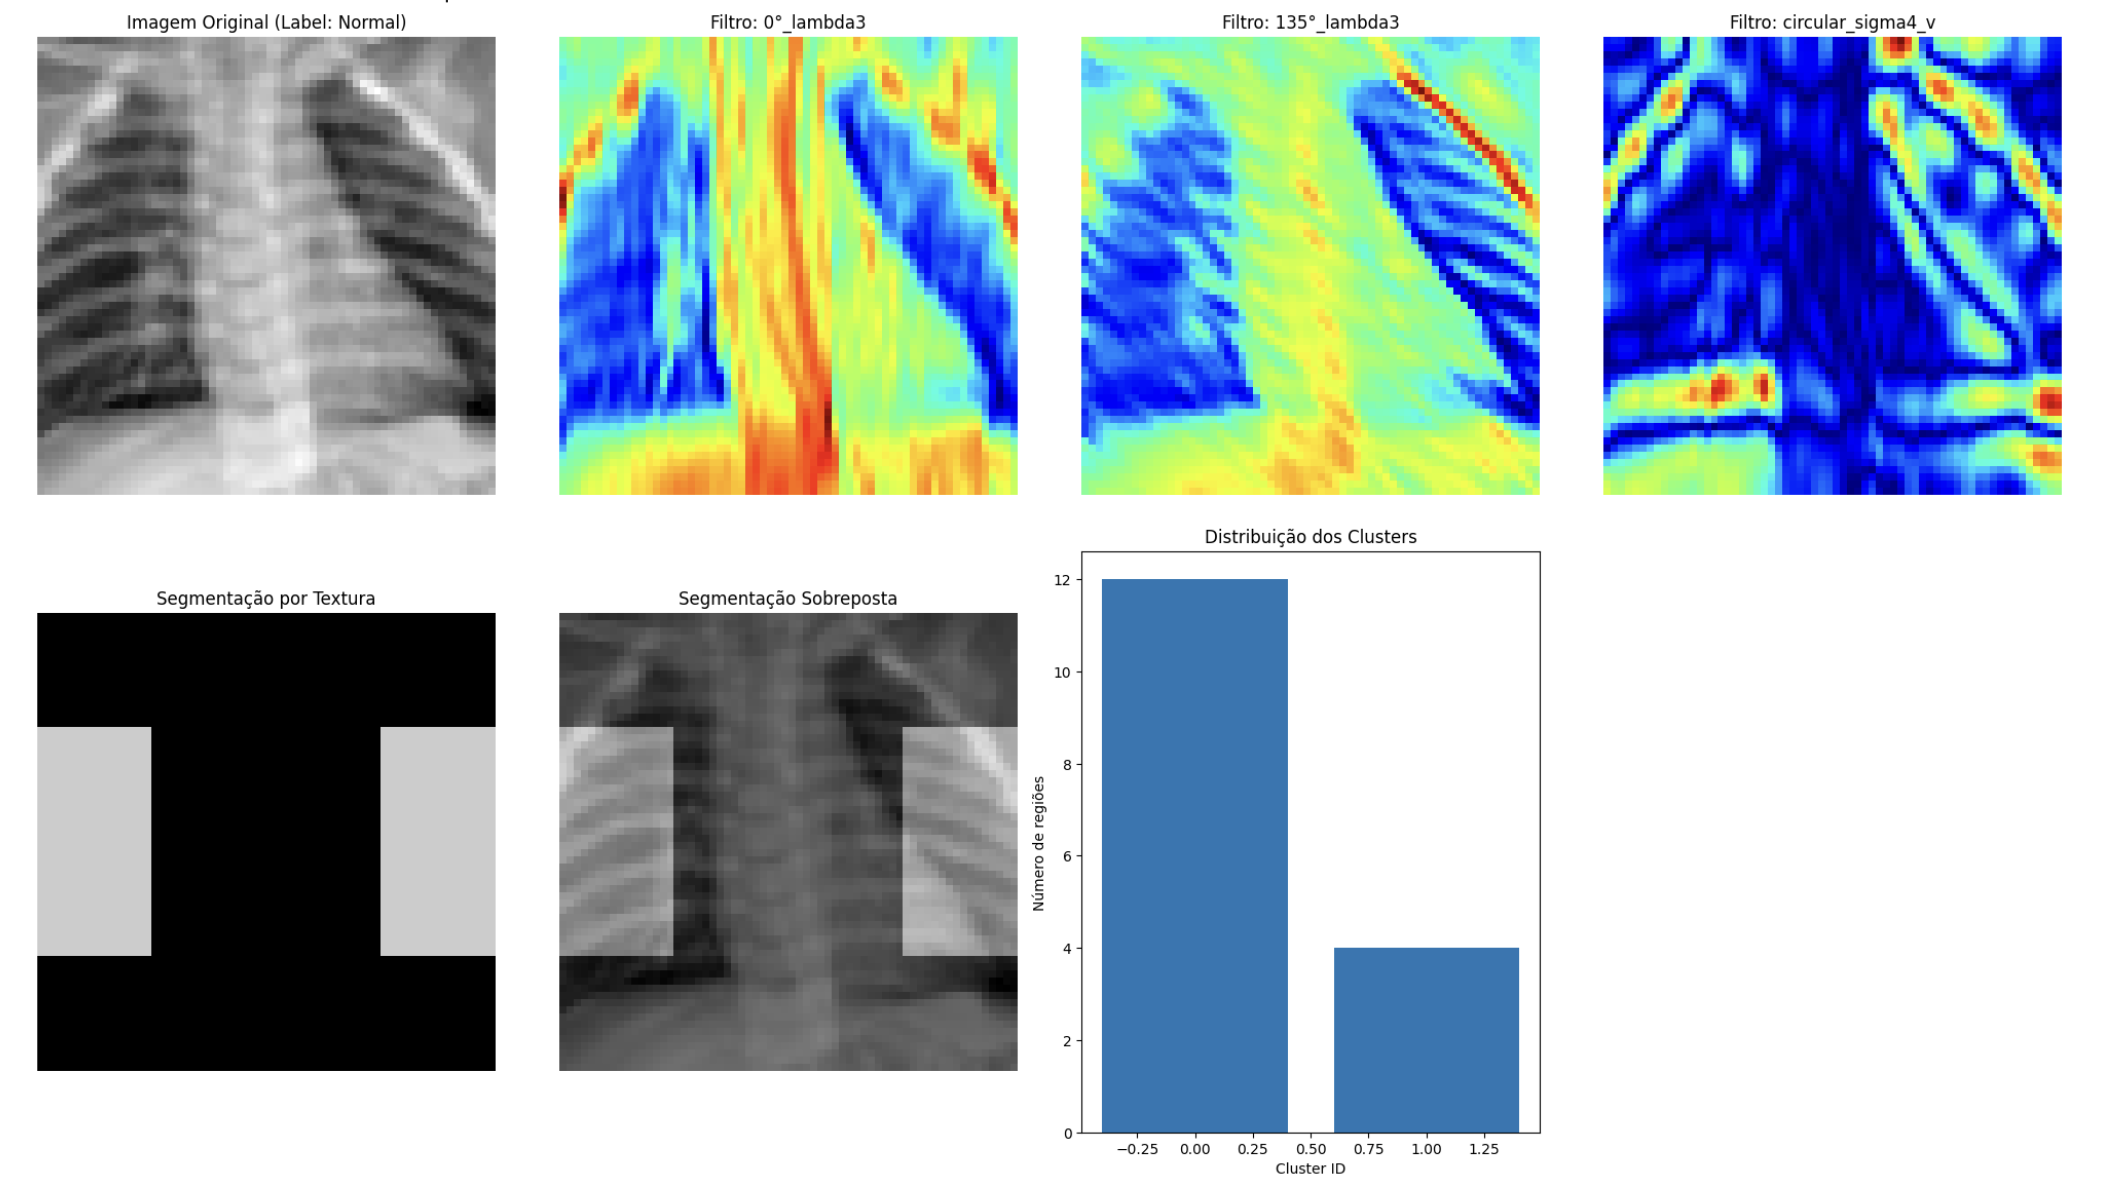
\includegraphics[width=1\linewidth]{../images/filtros_normal.png}
  \caption{Respostas dos filtros de Gabor e LoG aplicados a uma imagem de raio-X normal.}
  \label{fig:filtros_normal}
\end{figure}

\subsection{Segmentação por Textura}
A aplicação dos filtros de Gabor e LoG nas imagens de raio-X revelou padrões texturais distintos entre casos normais e casos de pneumonia. Os filtros de Gabor com orientações horizontais (0°) e diagonais (135°) mostraram-se particularmente eficazes na detecção de opacidades pulmonares características da pneumonia.

A figura \ref{fig:filtros_pneumonia} ilustra a aplicação dos filtros em uma imagem de raio-X com pneumonia, mostrando as respostas dos filtros de Gabor em diferentes orientações e escalas, bem como do filtro LoG. Podemos observar que os filtros ressaltam diferentes características texturais da imagem, permitindo uma análise mais detalhada das estruturas presentes.

\begin{figure}[h]
  \centering
  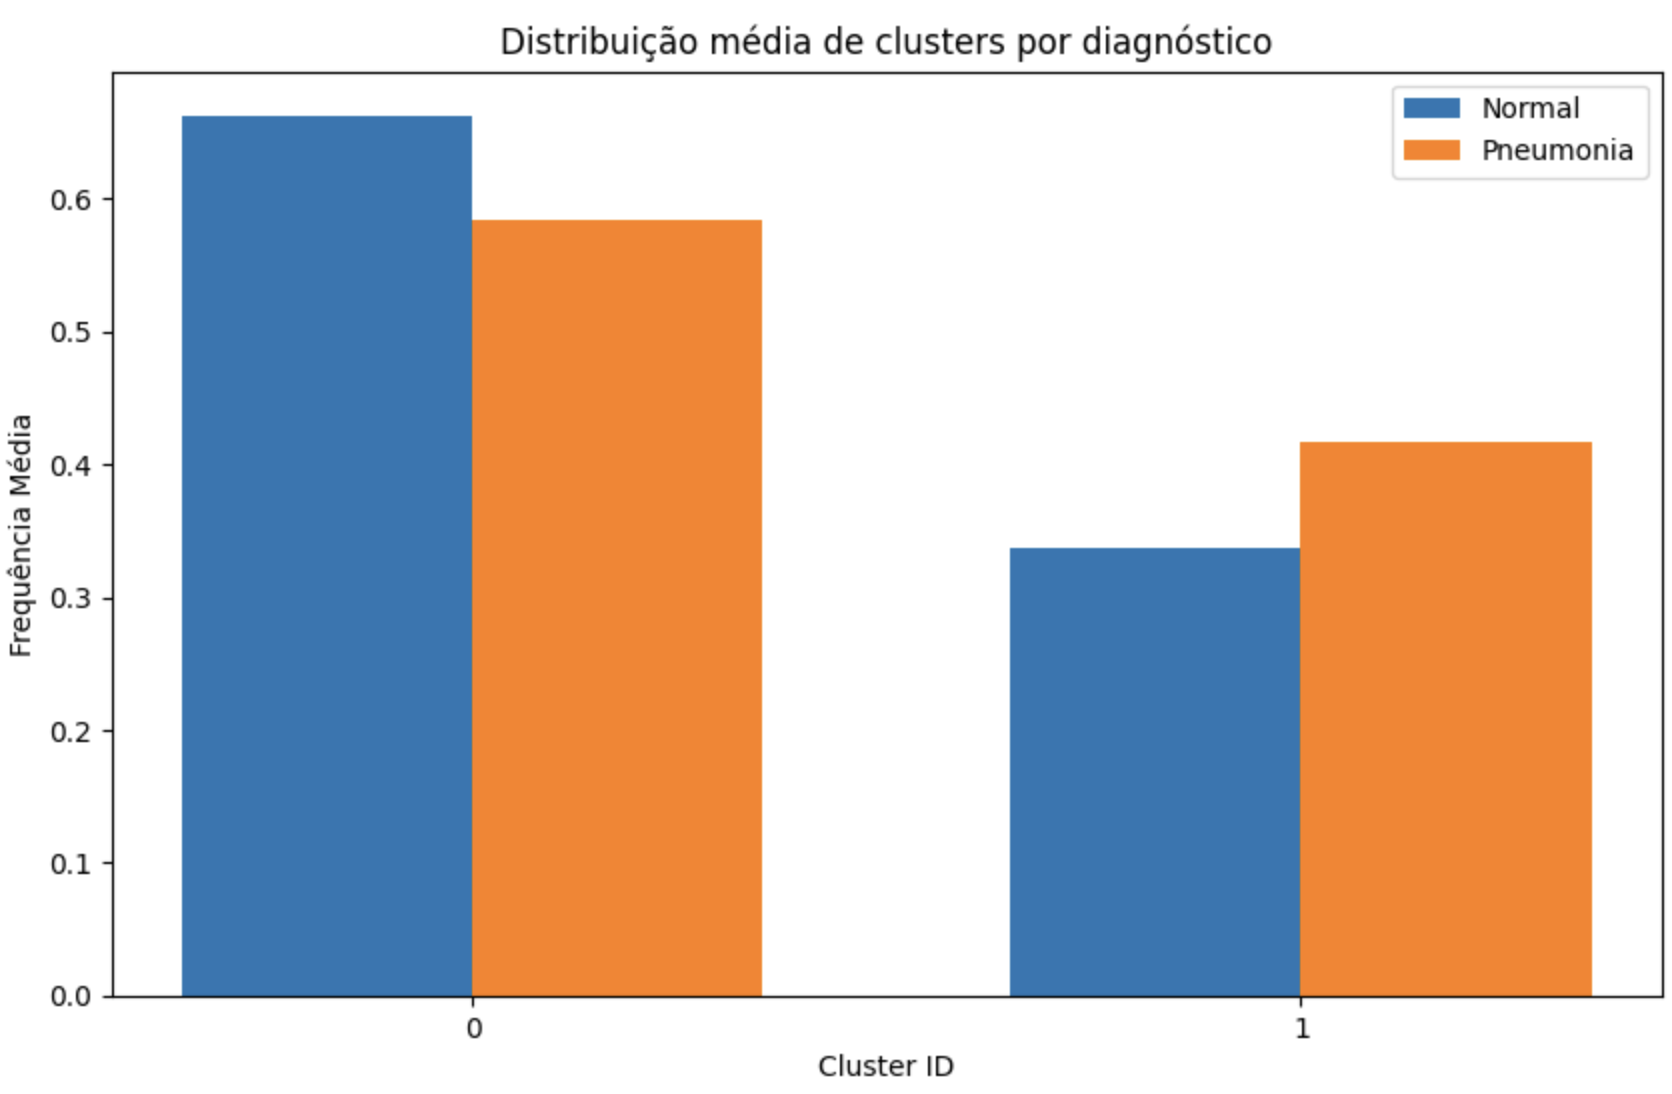
\includegraphics[width=0.8\linewidth]{../images/cluster_distribution.png}
  \caption{Distribuição dos clusters obtidos pela segmentação K-means em imagens normais e com pneumonia.}
  \label{fig:clusters}
\end{figure}
  
Em particular, observamos que:

\begin{itemize}
  \item Imagens com pneumonia apresentam maior prevalência do cluster 1, associado a regiões com alta resposta aos filtros de Gabor orientados a 45° e 135°, característicos das opacidades irregulares da pneumonia.
  \item Imagens normais apresentam maior prevalência do cluster 0, associado a regiões com baixa resposta a todos os filtros, indicando áreas pulmonares saudáveis.
\end{itemize}

\subsection{Comparação entre Abordagens Multi-escala}

A comparação entre as duas abordagens multi-escala implementadas mostrou que:

\begin{itemize}
  \item A abordagem de filtros em múltiplas escalas fornece uma representação mais detalhada das texturas locais, sendo mais eficaz na detecção de pequenas anomalias.
  \item A abordagem de pirâmide de imagens captura melhor as características globais e padrões de larga escala, sendo mais robusta a variações de posicionamento e tamanho das estruturas anatômicas.
\end{itemize}

// TODO: Revisar texto a seguir
A análise quantitativa da correlação entre os padrões de cluster e o diagnóstico revelou uma associação significativa entre determinados padrões texturais e a presença de pneumonia. Os clusters associados a regiões com alta resposta aos filtros de Gabor em orientações diagonais (45° e 135°) mostraram-se positivamente correlacionados com o diagnóstico de pneumonia, com uma diferença média de frequência de 0,18 entre casos normais e casos de pneumonia.

\subsection{Avaliação Quantitativa}
Nesta subseção apresentamos a avaliação quantitativa do classificador baseado em K-Means global, utilizando a matriz de confusão e as principais métricas de desempenho.

\begin{table}[h]
  \centering
  \caption{Matriz de Confusão no conjunto de teste}
  \label{tab:confusion_matrix}
  \begin{tabular}{lcc}
    \toprule
                   & \textbf{Previsto Normal} & \textbf{Previsto Pneumonia} \\
    \midrule
    \textbf{Real Normal}     & 74 (VN)   & 9  (FP)  \\
    \textbf{Real Pneumonia}  & 30 (FN)   & 87 (VP)  \\
    \bottomrule
  \end{tabular}
\end{table}

A partir da Tabela~\ref{tab:confusion_matrix}, calculamos:

\[
\text{Acurácia} = \frac{\text{VP} + \text{VN}}{\text{VP} + \text{VN} + \text{FP} + \text{FN}}
= \frac{87 + 74}{87 + 74 + 9 + 30} = 80{,}50\%
\]

Além da acurácia, outras métricas podem ser obtidas, por exemplo:
\[
\text{Precisão} = \frac{\text{VP}}{\text{VP} + \text{FP}}
= \frac{87}{87 + 9} \approx 90{,}58\%
\]
\[
\text{Sensibilidade (Recall)} = \frac{\text{VP}}{\text{VP} + \text{FN}}
= \frac{87}{87 + 30} \approx 74{,}35\%
\]
\[
\text{Especificidade} = \frac{\text{VN}}{\text{VN} + \text{FP}}
= \frac{74}{74 + 9} \approx 89{,}16\%
\]

Esses resultados mostram que o modelo apresenta boa precisão na detecção de pneumonia, embora a sensibilidade ainda possa ser melhorada em trabalhos futuros.

\subsection{Robustez e Limitações}

\begin{itemize}
  \item \textbf{Robustez:}
    \begin{itemize}
      \item Extração de textura com filtros de Gabor e LoG mantém estabilidade frente a variações moderadas de parâmetros (escalas, orientações, tamanho de janela).
      \item Padronização Z-score assegura comparabilidade das características mesmo sob diferentes níveis de brilho e contraste.
      \item Agrupamento por K-Means global preserva os padrões texturais principais sem demandar reparametrizações frequentes.
    \end{itemize}
  \item \textbf{Limitações:}
    \begin{itemize}
      \item Número de clusters fixo em 2 restringe a captura de padrões texturais mais finos.
      \item Treinamento global de K-Means sobre todos os patches exige crescente custo computacional conforme aumenta o volume de dados.
      \item Validação restrita ao PneumoniaMNIST, sem testes em outras modalidades de imagem médica.
      \item Desempenho sensível às escolhas de tamanho de janela e orientações dos filtros, exigindo calibração cuidadosa.
    \end{itemize}
\end{itemize}


\section{Discussão}

Os resultados obtidos neste estudo destacam a importância da análise de textura para a classificação de imagens médicas, especificamente no diagnóstico de pneumonia a partir de raios-X de tórax. A abordagem baseada em filtros de Gabor e LoG, combinada com segmentação por clustering, mostrou-se eficaz na identificação de padrões texturais associados à pneumonia.

\subsection{Interpretabilidade dos Resultados}

Uma vantagem significativa da abordagem proposta é a interpretabilidade dos resultados. Ao contrário de métodos de aprendizado profundo que funcionam como "caixas pretas", nossa abordagem permite visualizar diretamente as características extraídas e entender como diferentes padrões texturais contribuem para o diagnóstico. Esta interpretabilidade é crucial em aplicações médicas, onde a confiança e a compreensão dos resultados pelos profissionais de saúde são essenciais.

A análise dos centroides dos clusters obtidos revela informações valiosas sobre as características texturais associadas à pneumonia. Os clusters predominantes em casos de pneumonia apresentam alta resposta a filtros de Gabor em orientações diagonais e escalas intermediárias, correspondendo às opacidades irregulares e padrões reticulares típicos da doença.

\subsection{Comparação com Métodos de Deep Learning}

Embora métodos baseados em redes neurais convolucionais (CNNs) frequentemente alcancem maior acurácia em tarefas de classificação de imagens médicas, nossa abordagem clássica oferece vantagens complementares:

\begin{itemize}
  \item \textbf{Requisitos computacionais reduzidos:} Os métodos propostos exigem significativamente menos recursos computacionais e dados de treinamento em comparação com abordagens de deep learning.
  \item \textbf{Interpretabilidade:} A abordagem baseada em filtros de textura fornece insights diretos sobre as características utilizadas para classificação.
  \item \textbf{Robustez a conjuntos de dados limitados:} Em cenários com poucos dados de treinamento, métodos clássicos podem superar abordagens de deep learning que tendem a overfitting.
\end{itemize}

\subsection{Limitações e Trabalhos Futuros}

Identificamos algumas limitações em nossa abordagem que podem ser abordadas em trabalhos futuros:
\begin{itemize}
  \item \textbf{Aprimoramento da segmentação:} A segmentação por clustering pode ser aprimorada com técnicas mais avançadas, como segmentação baseada em aprendizado profundo.
  \item \textbf{Integração com métodos de deep learning:} A combinação de métodos clássicos e modernos pode resultar em um sistema de classificação mais robusto e preciso.
  \item \textbf{Avaliação em outros conjuntos de dados:} A validação da abordagem proposta em outros conjuntos de dados médicos pode fornecer insights adicionais sobre sua aplicabilidade e generalização.
\end{itemize}

\section{Conclusão}

Este trabalho investigou o uso de métodos clássicos de processamento de imagem, especificamente filtros de textura e segmentação por clustering, para a classificação de imagens médicas. Utilizando o dataset PneumoniaMNIST, demonstramos que a análise de textura baseada em filtros de Gabor e LoG pode extrair características relevantes para o diagnóstico de pneumonia em raios-X de tórax.

Os resultados revelaram padrões texturais distintos entre casos normais e casos de pneumonia, com diferenças significativas na distribuição de clusters obtidos pela segmentação. A análise multi-escala, implementada tanto por filtros em múltiplas escalas quanto por pirâmide de imagens, permitiu capturar características texturais em diferentes níveis de detalhe.

Embora os métodos clássicos possam não alcançar a acurácia de abordagens de deep learning em grandes conjuntos de dados, eles oferecem vantagens importantes em termos de interpretabilidade, requisitos computacionais e desempenho em cenários com dados limitados. A combinação de métodos clássicos e modernos representa um caminho promissor para o desenvolvimento de sistemas de auxílio ao diagnóstico médico que sejam precisos, interpretáveis e confiáveis.

\balance
\bibliographystyle{ACM-Reference-Format}
\bibliography{references}

\end{document}